\documentclass[dvisvgm,tikz,border=4pt]{standalone}
\usepackage{amsmath,amssymb}
\usepackage{pgfplots}\pgfplotsset{compat=1.18}\usepgfplotslibrary{polar}
\usetikzlibrary{arrows.meta,positioning,automata,shapes,shapes.misc,calc,decorations.pathmorphing,decorations.markings,angles,quotes,patterns,mindmap,matrix,knots,hobby,trees}
\tikzset{->-/.style={decoration={markings, mark=at position 0.5 with {\arrow{Stealth}}}, postaction={decorate}}}
\begin{document}
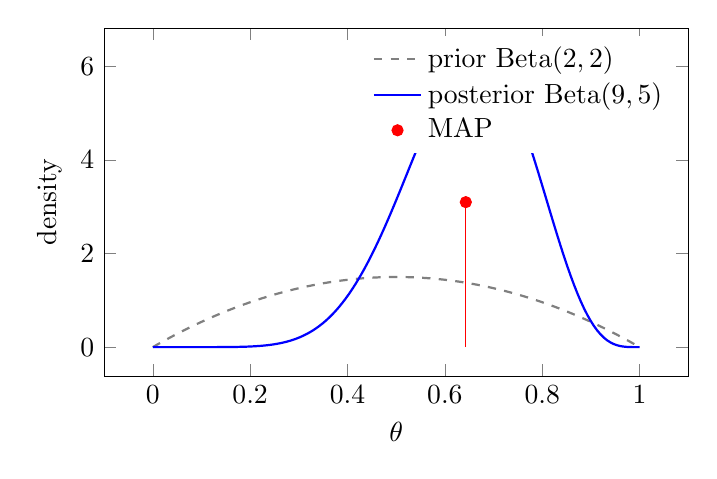
\begin{tikzpicture}
\begin{axis}[domain=0:1, samples=150, xlabel=$\theta$, ylabel={density}, width=9cm, height=6cm, legend cell align=left, legend style={draw=none}]
\addplot[gray, dashed, thick] {6*x*(1-x)}; \addlegendentry{prior $\mathrm{Beta}(2,2)$}
\addplot[blue, thick] {x^8*(1-x)^4/0.0000777}; \addlegendentry{posterior $\mathrm{Beta}(9,5)$}
\addplot[red, ycomb, mark=*, samples at={0.643}] {3.1}; \addlegendentry{MAP}
\end{axis}
\end{tikzpicture}
\end{document}
